\begin{figure}[h]
    \vspace*{0.3cm}
    \tikzset{every picture/.style={line width=0.75pt}} %set default line width to 0.75pt
    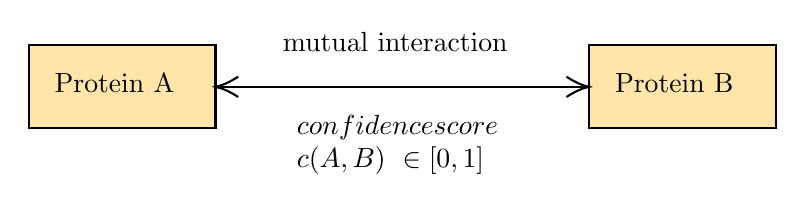
\begin{tikzpicture}[x=0.75pt,y=0.75pt,yscale=-1,xscale=1]
        %uncomment if require: \path (0,136); %set diagram left start at 0, and has height of 136

        %Shape: Rectangle [id:dp8315683426496481]
        \draw  [fill={rgb, 255:red, 255; green, 229; blue, 168 }  ,fill opacity=1 ] (20,20) -- (110,20) -- (110,60) -- (20,60) -- cycle ;
        %Shape: Rectangle [id:dp6227729030936355]
        \draw  [fill={rgb, 255:red, 255; green, 229; blue, 168 }  ,fill opacity=1 ] (290,20) -- (380,20) -- (380,60) -- (290,60) -- cycle ;
        %Straight Lines [id:da5202946805882411]
        \draw    (112,40) -- (288,40) ;
        \draw [shift={(290,40)}, rotate = 180] [color={rgb, 255:red, 0; green, 0; blue, 0 }  ][line width=0.75]    (10.93,-4.9) .. controls (6.95,-2.3) and (3.31,-0.67) .. (0,0) .. controls (3.31,0.67) and (6.95,2.3) .. (10.93,4.9)   ;
        \draw [shift={(110,40)}, rotate = 0] [color={rgb, 255:red, 0; green, 0; blue, 0 }  ][line width=0.75]    (10.93,-4.9) .. controls (6.95,-2.3) and (3.31,-0.67) .. (0,0) .. controls (3.31,0.67) and (6.95,2.3) .. (10.93,4.9)   ;

        % Text Node
        \draw (31,32) node [anchor=north west][inner sep=0.75pt]   [align=left] {Protein A};
        % Text Node
        \draw (301,32) node [anchor=north west][inner sep=0.75pt]   [align=left] {Protein B};
        % Text Node
        \draw (141,12) node [anchor=north west][inner sep=0.75pt]   [align=left] {mutual interaction};
        % Text Node
        \draw (141,50.4) node [anchor=north west][inner sep=0.75pt]    {$ \begin{array}{l}
                                                                              \text{confidence score}\\
                                                                              c( A,B) \ \in [ 0,1]
        \end{array}$};


    \end{tikzpicture}
    \caption{Schematic of an interaction between two proteins}
\end{figure}
